Trong chương này, tôi sẽ xây dựng hai kịch bản để kiểm thử hoạt động của phần mềm  IDS-DDoS trong mạng SDN. Hai kịch bản này là:

\begin{itemize}
	\item [--] Mạng SDN bị tấn công từ bên ngoài. Kịch bản này tương tự như các kịch bản tấn công mạng thường gặp. Trong trường hợp này, tôi sẽ sử dụng IDS-DDoS để cố gắng bảo vệ và giảm thiểu thiệt hại cho hệ thống mạng cũng như máy chủ web bên trong.
	\item [--] Máy con trong mạng SDN bị lợi dụng tấn công ra bên ngoài. Kịch bản này tương tự như kịch bản các thiết bị IoT bị xâm nhập và trở thành botnet. Trong trường hợp này, tôi sẽ cố gắng ngăn chặn các thiết bị bên trong mạng SDN thực hiện tấn công đến các máy chủ bên ngoài.
\end{itemize}

Với phần  mềm IDS-DDoS, tôi sử dụng mô hình LSVM để nhận diện các luồng tấn công. Mặc dù kết quả huấn luyện cho thấy LSVM có độ chính xác thấp hơn so với Decision Tree, Random Forest hay DNN (mục \ref{compare-multi-models}), tuy nhiên, khi áp dụng thực tế, LSVM lại nhận diện luồng tấn công tốt hơn. Kết luận này được tôi rút ra từ việc quan sát quá trình hoạt động của các mô hình trong môi trường thực nghiệm, phần này sẽ được tôi trình bày trong phần \ref{test-conclusion}.

Các biểu đồ trong mục này được chụp từ công cụ theo dõi lưu lượng gói tin trong mạng được thiết kế trong mục \ref{traffic-monitor}.

\section{Mạng SDN bị tấn công từ bên ngoài}
\label{c:6.1}

Trong kịch bản này, Outer Attacker sẽ sử dụng công cụ HOIC để tấn công vào Webserver H2.

Giao diện công cụ HOIC trong hình \ref{fig:hoic}. Vì đây là công cụ không dành cho học thuật và có thể bị lợi dụng để sử dụng với mục đích xấu  nên tôi không chỉ ra nơi tham khảo hay cách tải xuống công cụ này.

\begin{figure}[ht!]
	\centering
	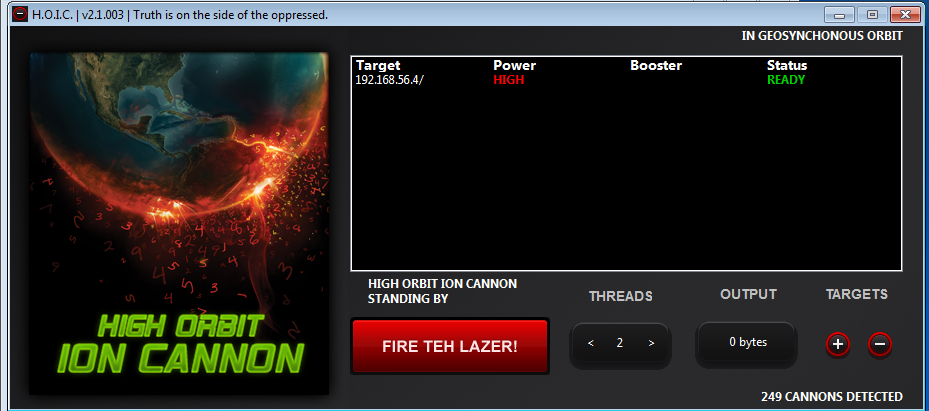
\includegraphics[width=0.75\linewidth]{fig/hoic.png}
	\caption{Giao diện công cụ HOIC}
	\label{fig:hoic}
\end{figure}

Quá trình tấn công được biểu thị trong các biểu đồ dưới đây.

Biểu đồ trong hình \ref{fig:B1} mô tả trạng thái mạng trước và trong lúc bị tấn công. 

Lúc đầu, nhìn theo trục gói tin, ta thấy được số lượng gói tin đến và gói tin đi vẫn còn thấp. Đường màu xanh lá biểu diễn số lượng gói tin đi, tức là các gói tin được phản hồi từ máy chủ web H2. Đường màu xanh dương biểu thị gói tin đến, tức là các gói tin được gửi tử Outer attacker.

Tuy nhiên, khi tấn công diễn ra, ta thấy được số lượng gói tin đến và đi tăng lên đột ngột trong một khoảng thời gian. Sau đó, số lượng gói tin đi (đường xanh lá) giảm xuống 0, trong khi số lượng gói tin đến (đường xanh dương) vẫn tăng. Nguyên nhân là do khi IDS-DDoS phát hiện tấn công và thông báo cho SDN  controller chặn luồng IP, lúc này, máy chủ H2 bên trong mạng không thể nhận thêm yêu cầu từ attacker nên không thể phản hồi, trong khi đó attacker vẫn tiếp tục tấn công làm cho số lượng gói tin đến tăng không ngừng.

\begin{figure}[ht!]
	\centering
	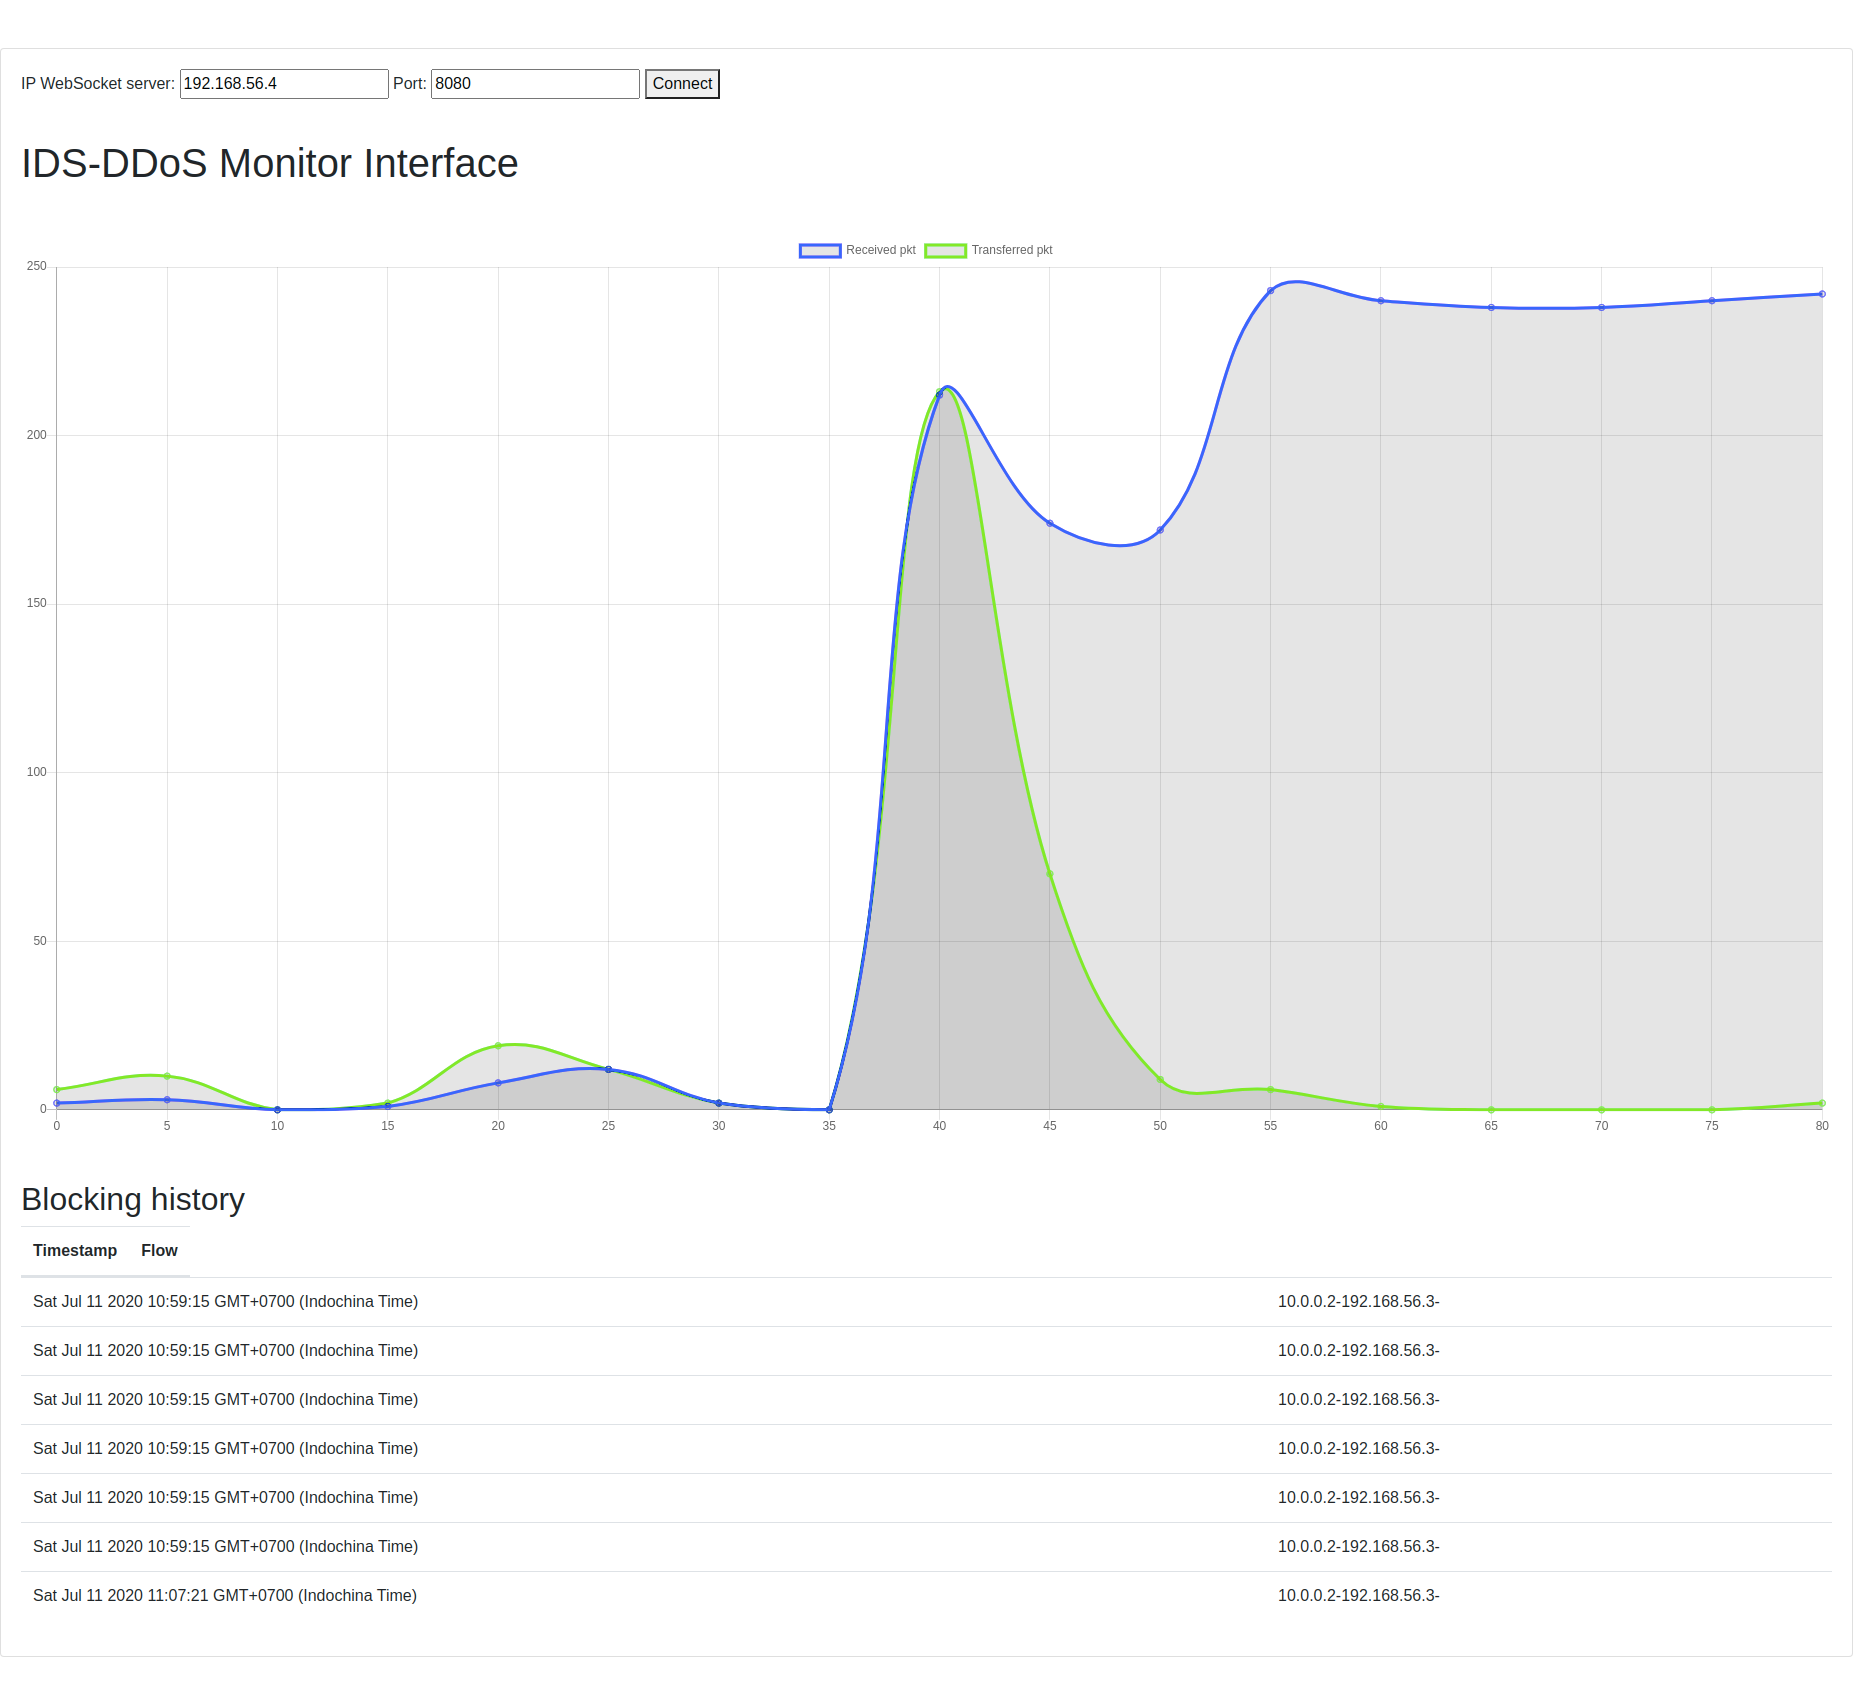
\includegraphics[width=\linewidth]{fig/B1.png}
	\caption{Kịch bản 1: Trạng thái mạng trước và trong khi tấn công}
	\label{fig:B1}
\end{figure}

Sau khi kết thúc tấn công (hình \ref{fig:B2}), số lượng gói tin đến và đi đều giảm xuống 0.

\begin{figure}[ht!]
	\centering
	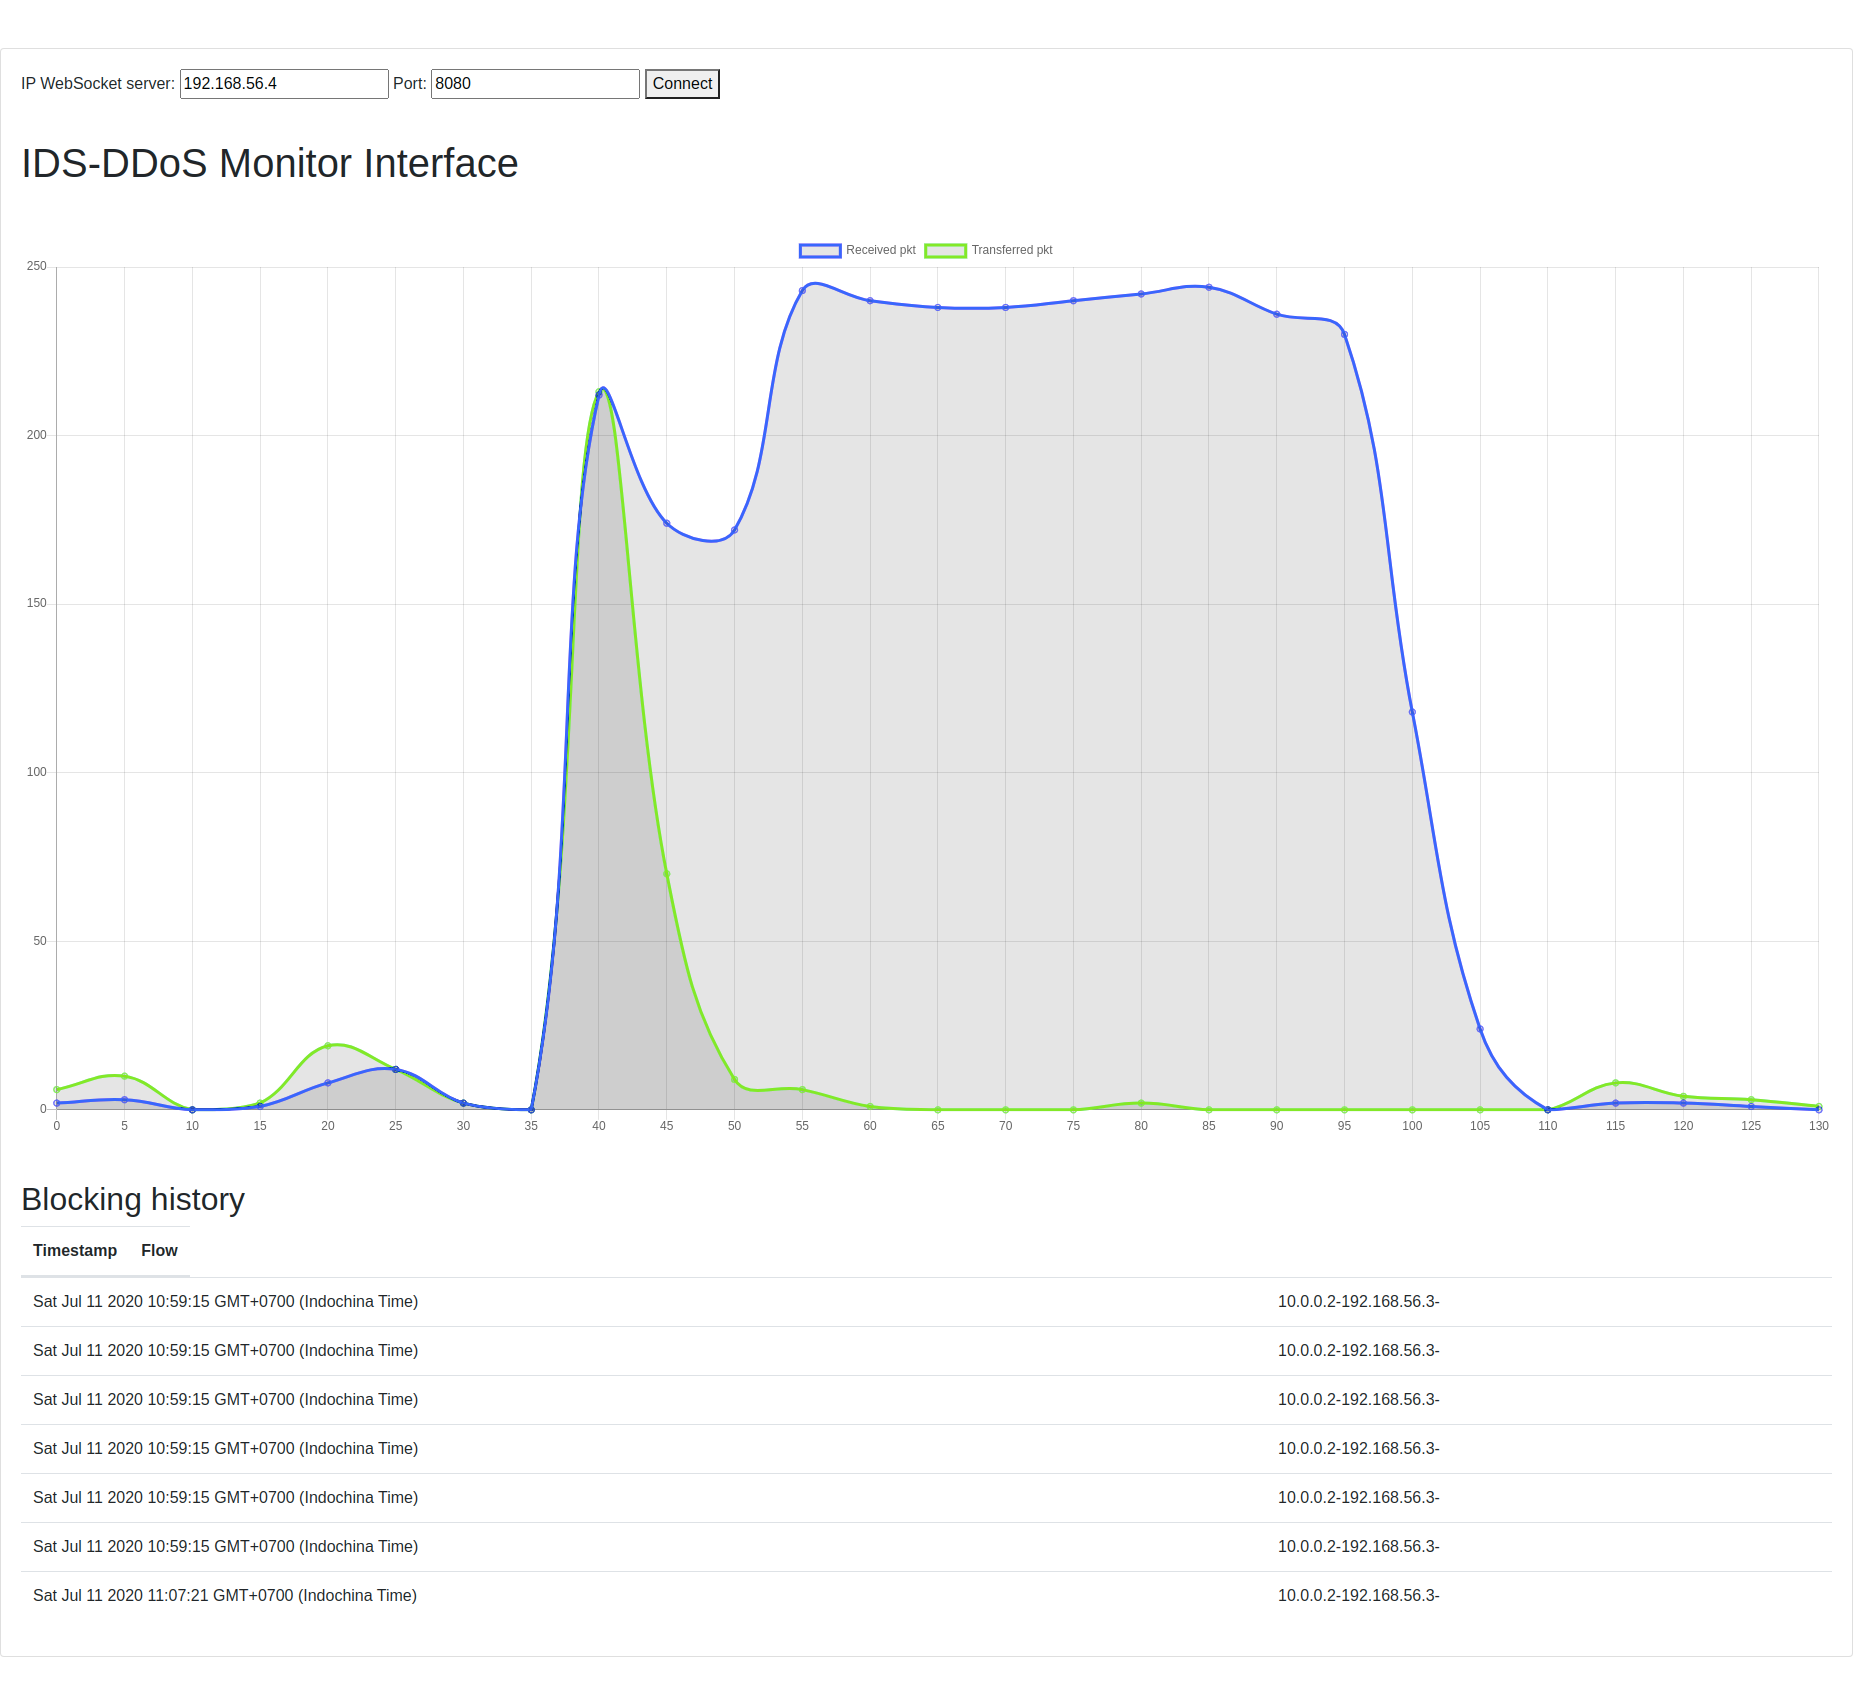
\includegraphics[width=\linewidth]{fig/B2.png}
	\caption{Kịch bản 1: Trạng thái mạng sau khi tấn công}
	\label{fig:B2}
\end{figure}

\section{Máy con trong mạng SDN bị lợi dụng tấn công ra bên ngoài}

Trong kịch bản này attacker H1 sẽ tấn công vào Outer Webserver bằng công cụ Hulk.

Hulk là công cụ giao diện console, với cùng lý do nêu trong mục \ref{c:6.1}, tôi cũng sẽ không chia sẽ cách tiếp cận công cụ này.

Quá trình tấn công được biểu thị trong biểu đồ \ref{fig:C1} dưới đây.

Lúc đầu, nhìn theo trục gói tin, ta thấy được số lượng gói tin đến và gói tin đi vẫn còn thấp.

Đường màu xanh dương biểu diễn gói tin đến, tức là các gói tin phản hồi từ Outer Webserver. Đường màu xanh lá biểu diễn gói tin đi, tức là các gói tin được gửi từ Attacker H1.

\begin{figure}[ht!]
	\centering
	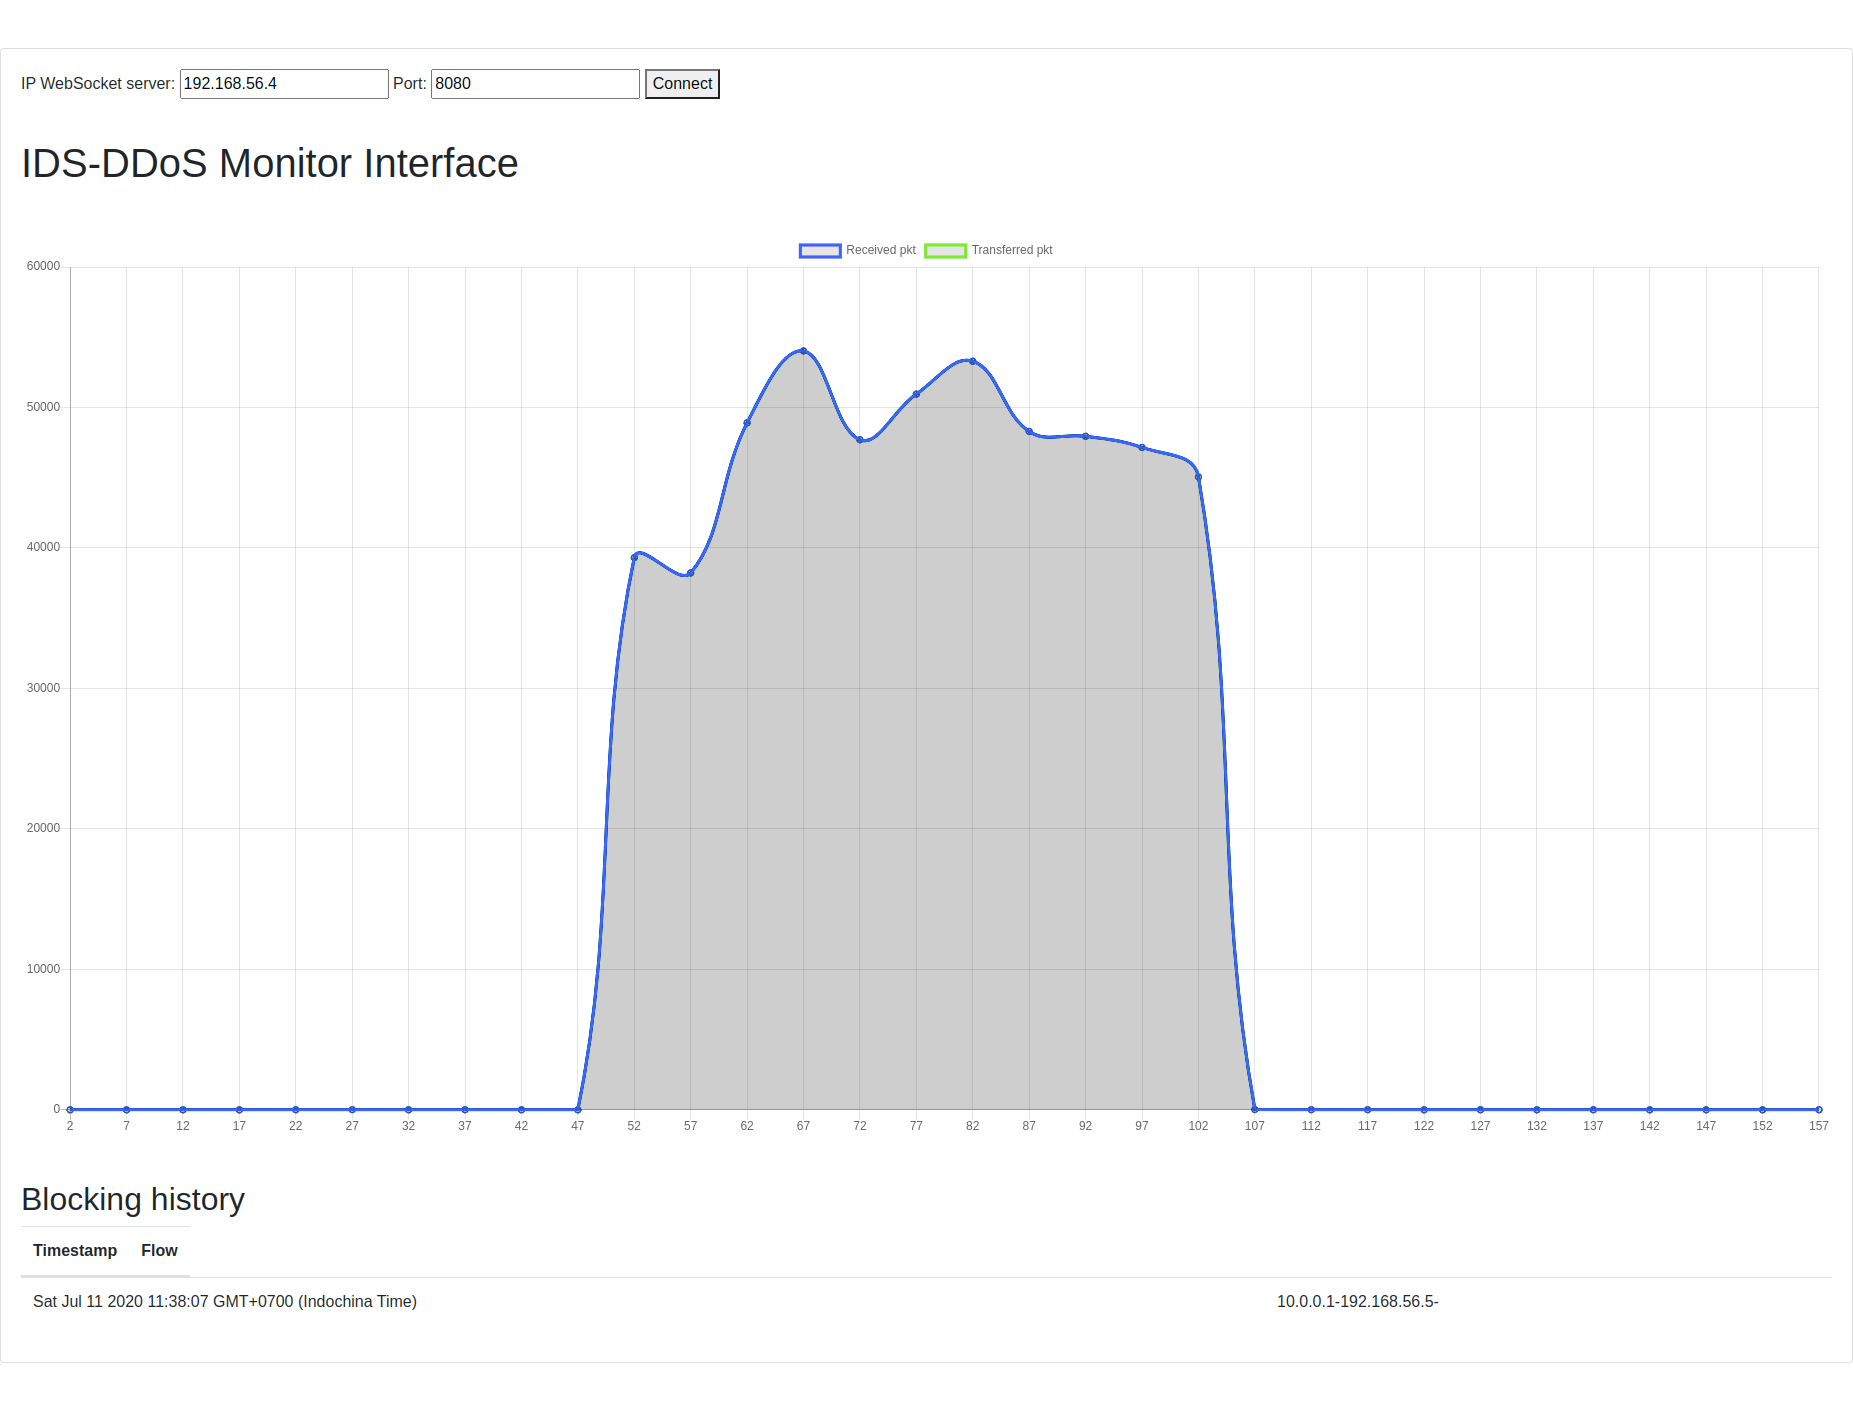
\includegraphics[width=\linewidth]{fig/C1.png}
	\caption{Kịch bản 2: Trạng thái mạng trong quá trình H1 tấn công}
	\label{fig:C1}
\end{figure}

Tuy nhiên, khi H1 bắt đầu tấn công, ta thấy số lượng gói tin đến và đi tăng lên đột ngột và tăng rất cao. Tuy nhiên sau một khoảng thời gian, số lượng gói tin này giảm xuống còn 0. Lý do là vì khi IDS-DDoS phát hiện tấn công và thông báo cho SDN controller để chặn luồng IP, cho nên H1 không thể tiếp tục tạo các kết nối đến Outer Webserver. Bên cạnh đó, H1 là máy con trong mạng SDN, nên các gói tin bị chặn tại nguồn tấn công, ta không thể quan sát được số lượng gói tin đi (đường xanh lá) tiếp tục tăng như trong kịch bản \ref{c:6.1} dù cho H1 vẫn tiếp tục tấn công.

\section{Kết luận kết quả kiểm thử}
\label{test-conclusion}

Từ hai kịch bản thí nghiệm trên, tôi nhận thấy phần mềm IDS-DDoS có khả năng nhận diện và phòng thủ trước tấn công DDoS. Tuy nhiên, khi so sánh giữa hai biểu đồ \ref{fig:B1} và \ref{fig:B2}, tôi nhận thấy, phần mềm không nhận diện tốt được các luồng tấn công từ công cụ Hulk.

Tôi đã tìm hiểu nguyên nhân và phát hiện ra rằng, trong dataset CICIDS2018 mà tôi sử dụng ở mục \ref{ids-dataset}, các luồng tấn công Hulk mà tác giả ghi nhận rất khác so với luồng tấn công do công cụ Hulk được tôi sử dụng. Trong đó, các gói tin và thời gian của luồng mà công cụ Hulk do tôi sử dụng sẽ nhỏ hơn nhiều so với tác giả. Lý do này đã khiến cho công cụ IDS-DDoS bị nhầm lẫn hầu hết các luồng tấn công Hulk là luồng hợp lệ. Thử nghiệm với mô hình học sâu DNN, tôi cũng được kết quả tương tự.

Ngoài ra, khi áp dụng các mô hình vào phần mềm IDS-DDoS trong môi trường thực nghiệm, tôi nhận ra vấn đề về khả năng nhận diện tấn công của các mô hình trong khi huấn luyện và trên thực tế là khá khác nhau.

Để xấy dựng môi trường thực nghiệm, tôi thiết kế một mạng gồm hai máy ảo, một máy đóng vai trò là ''attacker'' một máy đóng vai trò là ''victim''. Trên máy victim tôi cài đặt phần mềm IDS-DDoS để nhận diện tấn công. Sau đó, tôi sử dụng công cụ HOIC để thực hiện giả lập tấn công DDoS từ máy attacker sang máy victim. 

Trong lúc thực nghiệm, mô hình Naive Bayes cho kết quả tệ nhất các luồng tấn công và luồng thông thường bị nhận diện nhầm rất nhiều. Tuy nhiên điều làm tôi ngạc nhiên là mặc dù có độ chính xác cao với kiến trúc đơn giản nhưng Decision Tree và Random Forest lại thể hiện khả năng nhận diện tấn công rất kém, hầu hết các luồng tấn công đều được nhận diện là luồng thông thường. Trong khi đó, mô hình LinearSVM và DNN tuy có các tiếp cận phức tạp hơn và độ chính xác không cao bằng, nhưng lại nhận diện rất tốt các luồng tấn công.

